\section{Results and Discussion}
\label{sec:results}

%TODO: check, at the very end, if chars are in the right place

\begin{center}
    \begin{tabular}{ |c|c||c|c| } 
        \hline
        \textbf{Index} & \textbf{Run} & \textbf{Map Score} & \textbf{NCDG Score}\\
        \hline\hline
        01 & en\_en & \cellcolor{red!30!white}0.0700 & \cellcolor{red!30!white}0.1614 \\
        \hline
        02 & en\_en\_en\_3gram & 0.0704 & 0.1661 \\
        \hline
        03 & en\_en\_4gram & 0.0874 & 0.2025 \\
        \hline
        04 & en\_en\_5gram & 0.1028 & 0.2288 \\
        \hline
        05 & en\_en\_fr\_5gram & \cellcolor{red!60!white}0.0669 & \cellcolor{red!60!white}0.1525 \\
        \hline
        06 & en\_en\_4gram\_ner & \cellcolor{red}0.0360 & \cellcolor{red}0.1098 \\
        \hline
        07 & fr\_fr & 0.1656 & 0.3135 \\
        \hline
        08 & fr\_fr\_3gram & \cellcolor{green!30!white}0.1698 & \cellcolor{green!30!white}0.3208 \\
        \hline
        09 & fr\_fr\_4gram & \cellcolor{green!60!white}0.1737 & \cellcolor{green!60!white}0.3269 \\
        \hline
        10 & fr\_fr\_5gram & \cellcolor{green}0.1748 & \cellcolor{green}0.3285 \\
        \hline
        11 & fr\_en\_fr\_5gram & 0.1288 & 0.2797 \\
        \hline
        12 & fr\_fr\_4gram\_ner & 0.1362 & 0.2881 \\
        \hline
    \end{tabular}
\end{center}

\begin{figure}[h!]
	\centering
	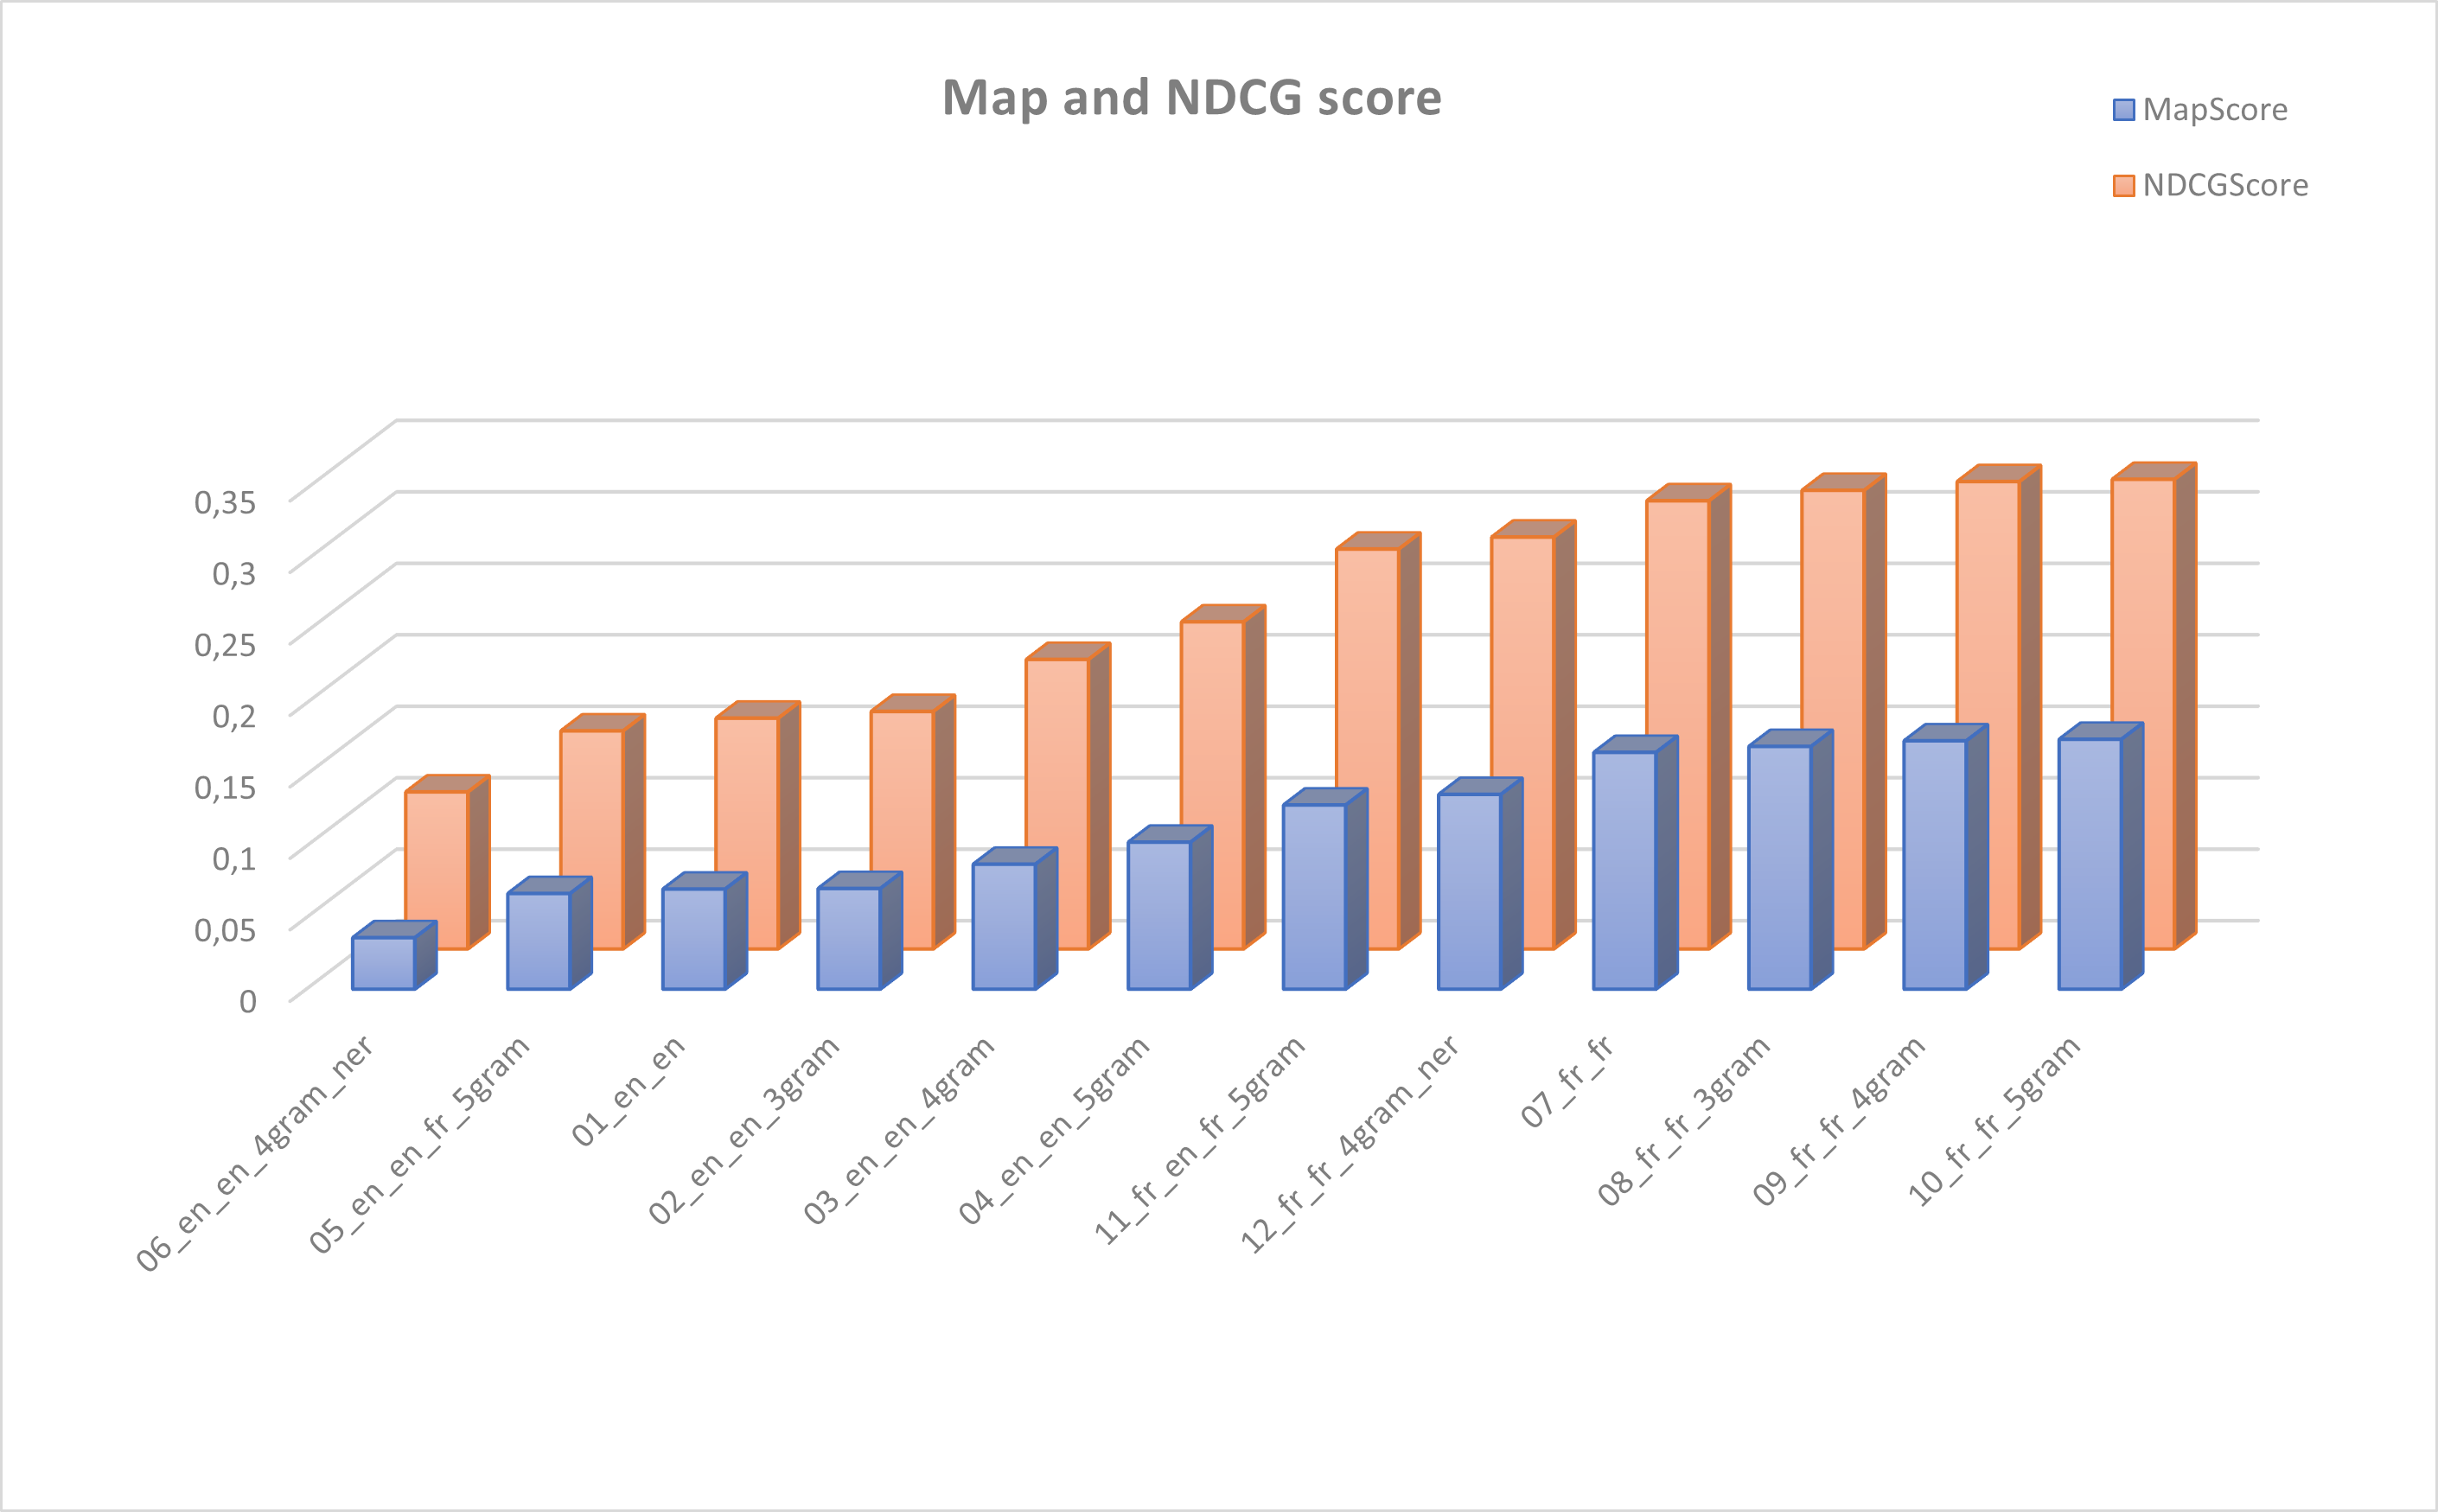
\includegraphics[width=0.7\textwidth]{figure/allScoresSorted.png}
	\caption{All scores sorted by MAP score}
	\label{fig:sorted scores}
\end{figure}
The dataset comprises MAP and NDCG scores for twelve runs of an Information Retrieval (IR) system with different language models and n-gram sizes for indexing. MAP measures how effectively the IR system returns relevant results for a given query, while NDCG indicates the ranking quality of the results.\\
The analysis shows that the highest MAP score (0.1748) is achieved by fr\_fr\_5gram, followed fr\_fr\_4gram (0.1737) and fr\_fr\_3gram (0.698), while the lowest MAP score (0.0360) is obtained by en\_en\_4gram\_ner. Similarly, the highest NDCG score (0.3208) belongs to fr\_fr\_4gram\_ner, followed by fr\_fr\_5gram (0.3285) and fr\_fr\_4gram (0.3269), whereas the lowest NDCG score (0.1098) corresponds to en\_en\_4gram\_ner.\\
Results suggest that French queries perform better than their English counterparts, possibly due to the training data's origin in
French and later translation into English. Moreover, the IR system's effectiveness generally increases with a larger n-gram size, as indicated by the higher scores of en\_en\_5gram and fr\_fr\_5gram. Conversely, the inclusion of named entity recognition (ner) in the indexing process seems to have a negative impact on the scores, as shown by the lower scores of en\_en\_4gram\_ner and fr\_fr\_4gram\_ner.\\
Here a chart ranking of five best scores, there are indexes that has been presented at CLEF:
\begin{figure}[h!]
	\centering
	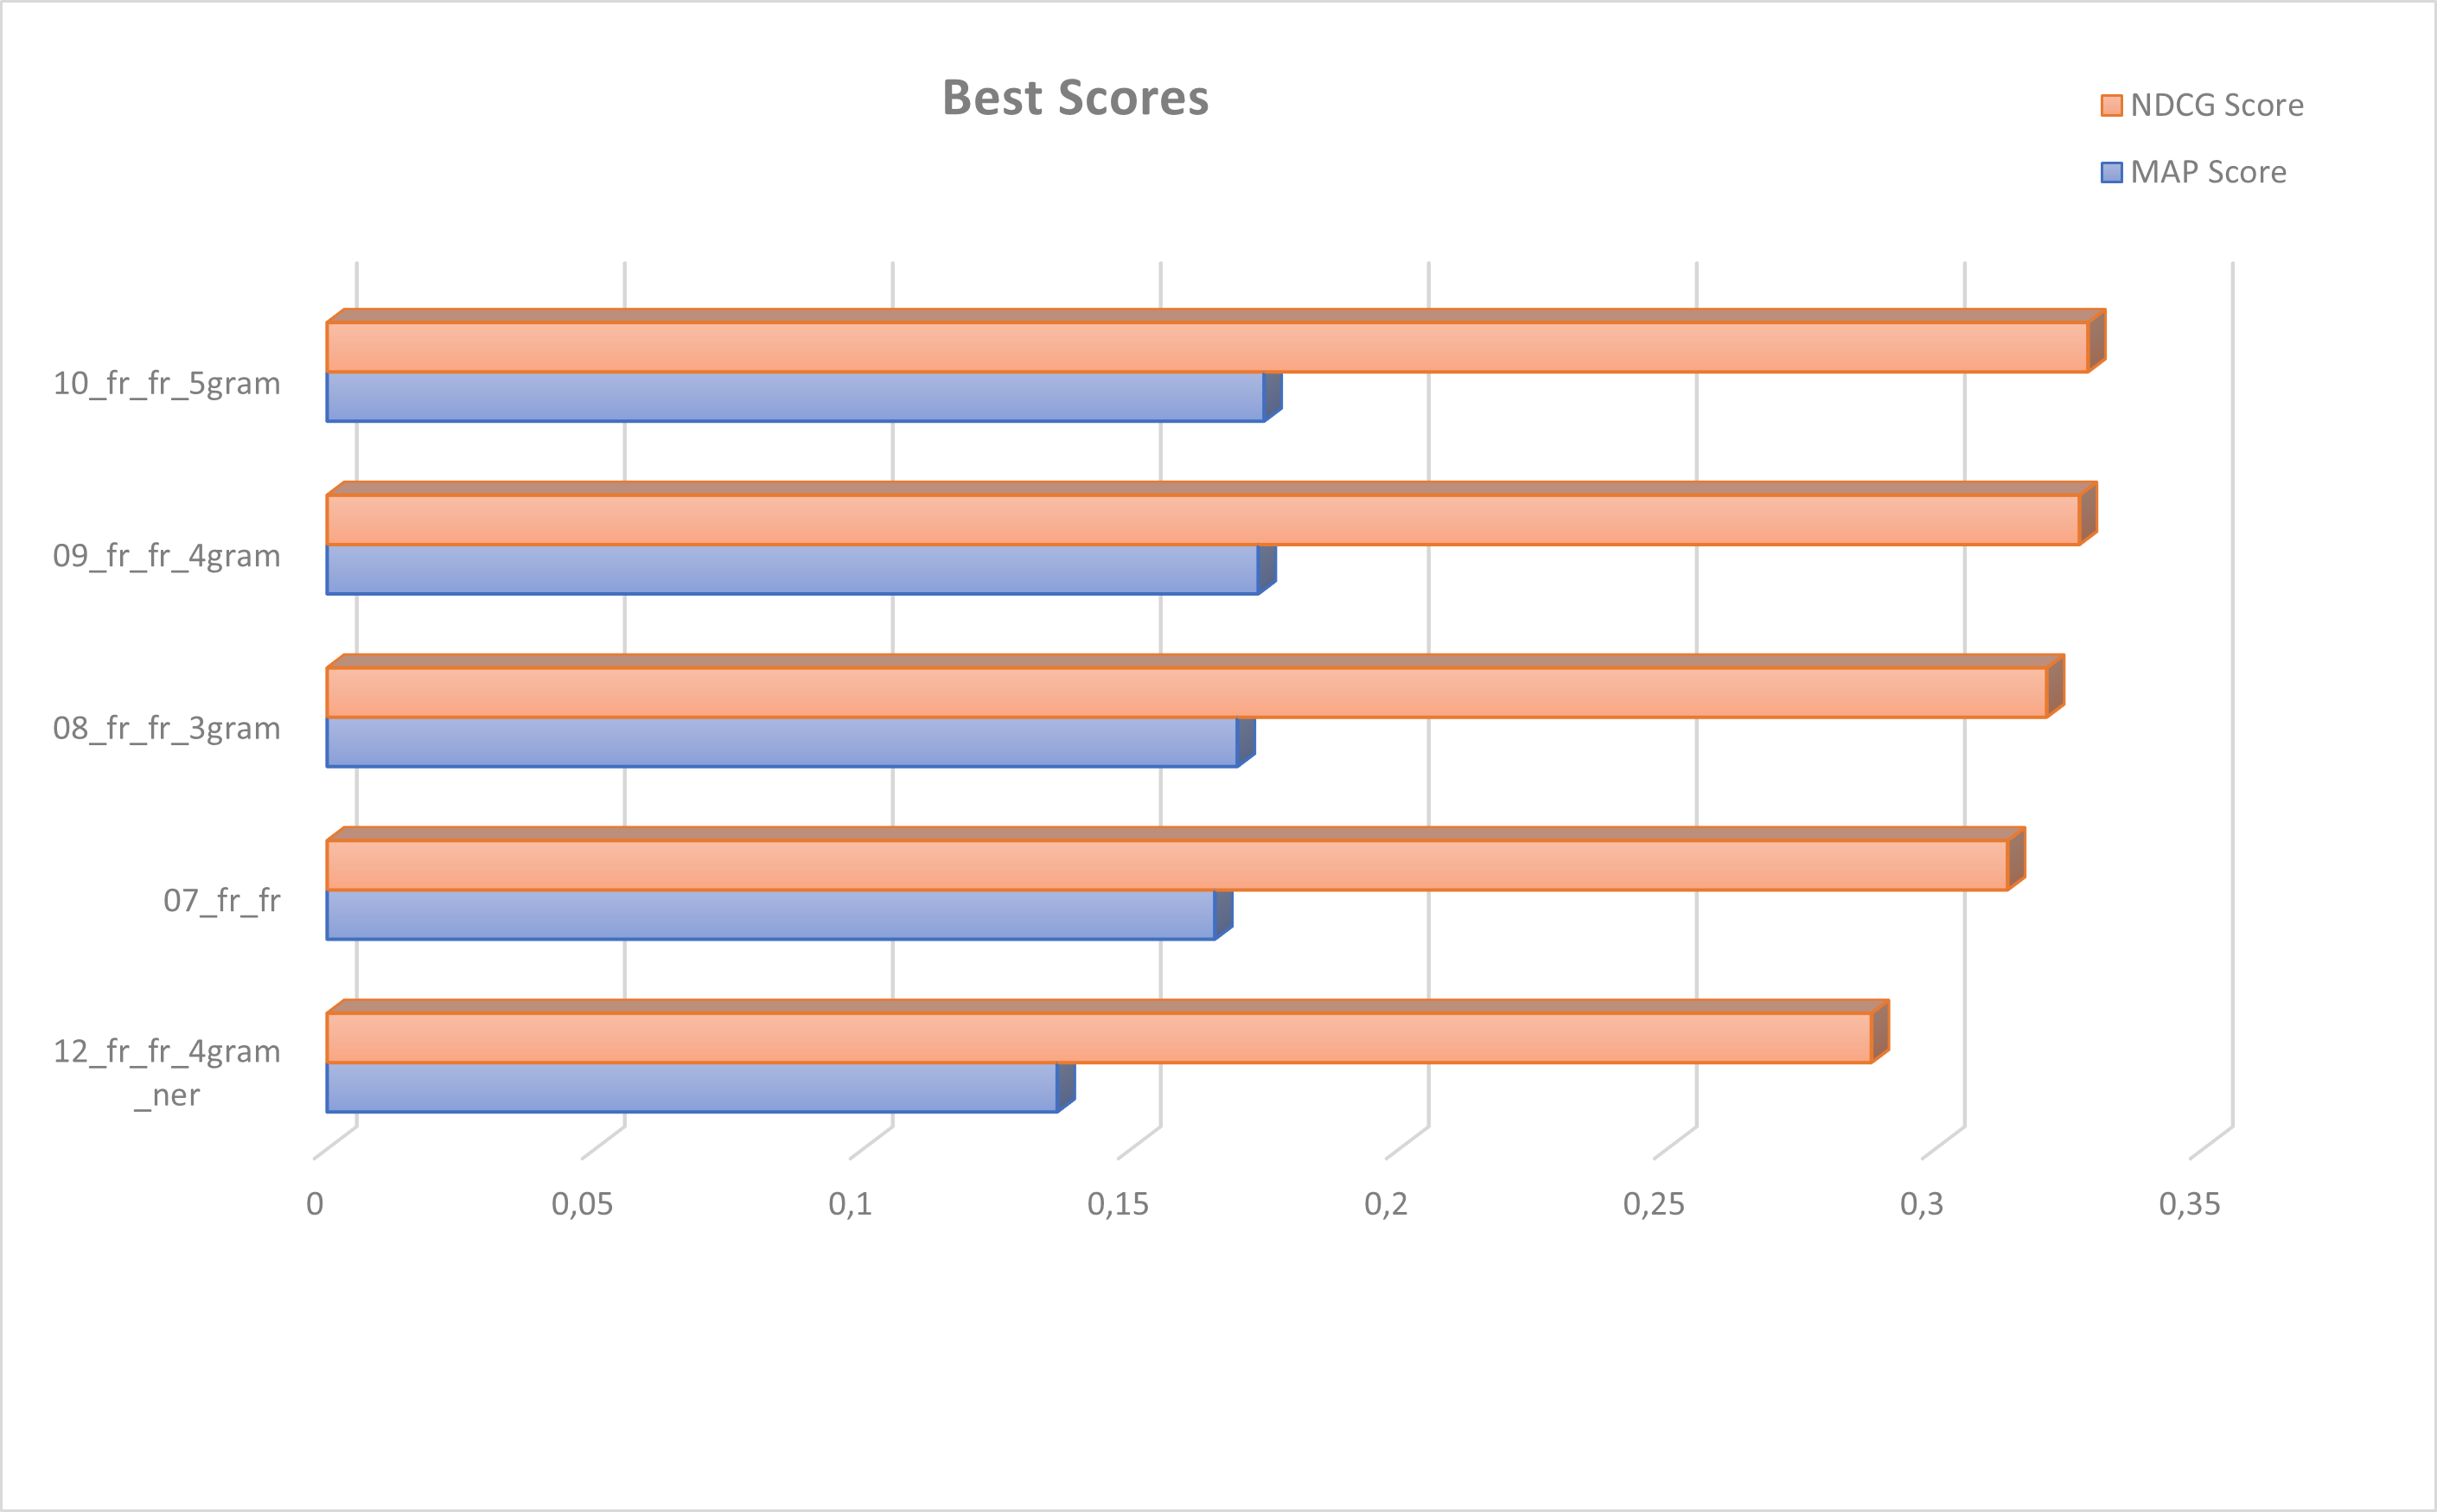
\includegraphics[width=0.7\textwidth]{figure/bestScores.png}
	\caption{Best MAP and NDCG scores}
	\label{fig:scores}
\end{figure}
It's interesting to notice that a cross-language approach (fr\_en\_fr\_5gram) is just out of the five bests performing indexes, even though it has english indexes. We suppose this is due to the fact that most of the score comes from the French queries, which are the most relevant ones.\\
On the other hand, the worst performing index is the one with named entity recognition (en\_en\_4gram\_ner): it combines translated queries and named entity recognition, which appears to be the two worst performing approaches.\\
In general, we focus more on trying multiple approaches, this is why our score has such a big space for improvement. As already said, French queries with bigger n-gram size perform better: queries weren't made by single word match, instead the more context was given, the better the results were.\\
